%%%%%%%%%%%%%%%%%%%%%%%%%%%%%%%%%%%%%%%%%%%%%%%%%%%%%%%%%%%%%%%%%%%%%%%%%%%%%%%%%%%%
% Document data
%%%%%%%%%%%%%%%%%%%%%%%%%%%%%%%%%%%%%%%%%%%%%%%%%%%%%%%%%%%%%%%%%%%%%%%%%%%%%%%%%%%%
\documentclass[12pt]{article} %report allows for chapters
%%%%%%%%%%%%%%%%%%%%%%%%%%%%%%%%%%%%%%%%%%%%%%%%%%%%%%%%%%%%%%%%%%%%%%%%%%%%%%%%%%%%
\usepackage{preamble}

\newcommand{\vecfieldB}{\boldsymbol{\vec{B}}}
\newcommand{\vecfieldE}{\boldsymbol{\vec{E}}}
\newcommand{\vecfieldJ}{\boldsymbol{\vec{J}}}
\newcommand{\grad}{\boldsymbol{\vec{\nabla}}}
\newcommand{\veclaplace}{\boldsymbol{\vec{\Delta}}}
\newcommand{\vecfieldV}{\boldsymbol{\vec{V}}}
\newcommand{\vecfieldA}{\boldsymbol{\vec{A}}}

\begin{document}

\begin{center}
   \textsc{\large MATH 272, Homework 10, \emph{Solutions}}\\
   \textsc{Due April 27$^\textrm{th}$}
\end{center}
\vspace{.5cm}

\begin{problem}
Consider the 1-dimensional wave equation given by
\[
\left(-\frac{\partial^2}{\partial x^2} +\frac{1}{c^2} \frac{\partial^2}{\partial  t^2} \right) u(x,t) = 0.
\]
We'll consider two distinct scenarios. First, we'll take an infinitely long elastic rod and second we'll take a rod of finite length with Dirichlet boundary conditions.
\begin{enumerate}[(a)]
    \item For a rod of infinite length, consider the initial conditions
    \[
    u(x,0) = \begin{cases} x+1 & -1\leq x \leq 0 \\ 1-x & 0\leq x \leq 1 \\ 0 & \textrm{otherwise} \end{cases} \qquad \textrm{and} \qquad \frac{\partial}{\partial t} u(x,0) = 0.
    \]
    Find and plot the portion of the wave that moves to the right with $c=1$.
    \item Let $u_R(x,t)$ be your solution from (a), show that this satisfies the right-moving wave equation
    \[
    \left(\frac{\partial}{\partial x} + \frac{1}{c} \frac{\partial}{\partial t} \right)u_R(x,t) = 0.
    \]
    \item Why is it that we can ignore the points where your function $u_R(x,t)$ is not differentiable even though we are considering this as a solution to a PDE?
    \item For an elastic rod $\Omega$ of finite length, $\Omega = [0,1]$, assume that we take the Dirichlet conditions $u(0,t)=0=u(1,t)$.  With the initial conditions
    \[
    u(x,0) = \sin(\pi x) \qquad \textrm{and} \qquad \frac{\partial}{\partial t} u(x,0)=0,
    \]
    find the solution using d'Alembert's formula.
    \item Let $w(x,t)$ be your solution for (d), show that it is indeed equal to
    \[
    w(x,t) = \sin(\pi x)\cos(\pi c t).
    \]
    \item With your result from (e), explain how we can decompose a standing wave into a linear combination of two waves; one moving towards the left and one moving towards the right and both reflecting off the boundary.
\end{enumerate}
\end{problem}
\begin{solution}~
\begin{enumerate}[(a)]
    \item We have that the solution is given by
\[
u(x,t) = \frac{1}{2} \left( u_L(x,t) + u_R(x,t)\right),
\]
where $u_L(x,t)$ is a portion of the wave moving to the left and $u_R(x,t)$ is the portion of the wave moving towards the right.  From our initial conditions, we have
\[
u_L(x,t) = \begin{cases} x+ct+1 & -1\leq x+ct \leq 0 \\ 1-x-ct & 0\leq x+ct \leq 1 \\ 0 & \textrm{otherwise} \end{cases} \qquad \textrm{and} \qquad u_R(x,t)=\begin{cases} x-ct+1 & -1\leq x-ct \leq 0 \\ 1-x+ct & 0\leq x-ct \leq 1 \\ 0 & \textrm{otherwise} \end{cases},
\]
which follows from d'Alembert's formula. 

We can then plot $u_R(x,t)$ for a few different times with $c=1$. 
\begin{figure}[H]
    \centering
    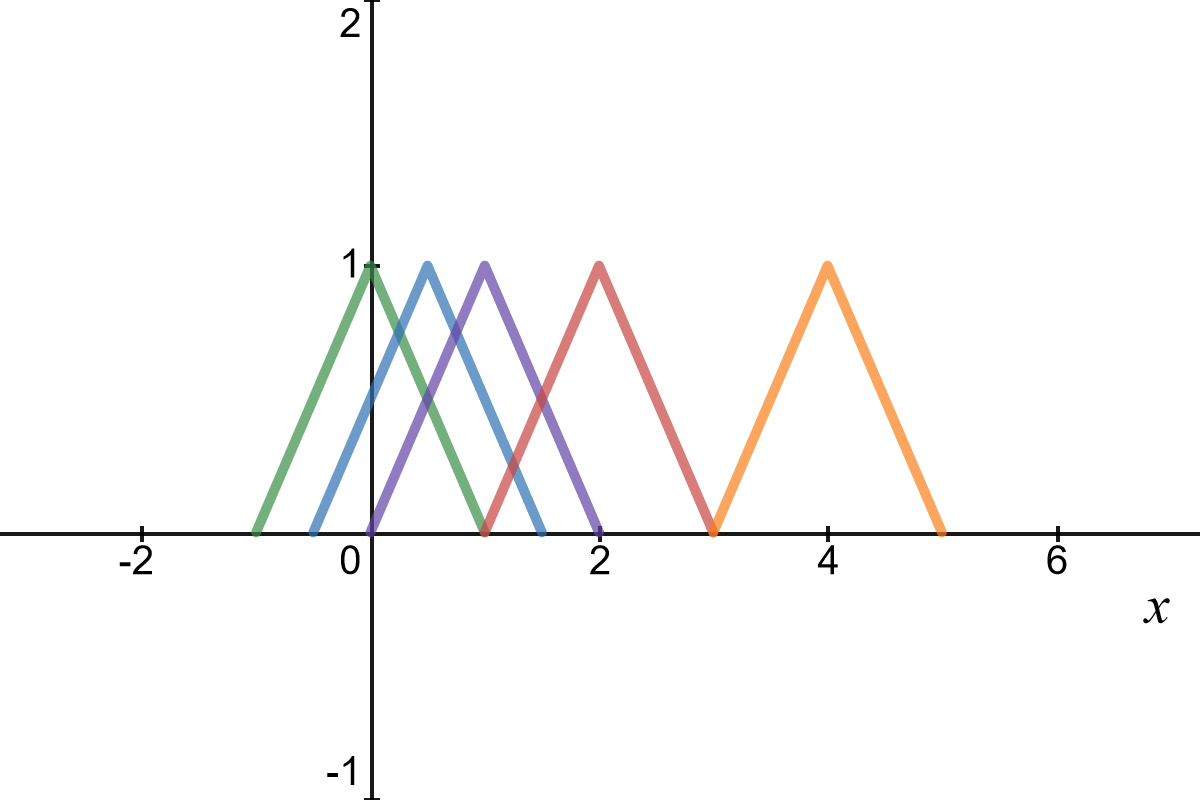
\includegraphics[width=.8\textwidth]{right_moving_triangle.png}
    \caption{Plots of $u_R$ for $t=0$ (green), $t=1/2$ (blue), $t=1$ (purple), $t=2$ (red), and $t=4$ (orange).}
\end{figure}
    \item We can take the derivatives of $u_R(x,t)$ to get
    \[
    \frac{\partial}{\partial x} u_R(x,t) = \begin{cases} 1 & -1< x-ct < 0 \\ -1 & 0<x-ct < 1 \\ 0 & \textrm{otherwise} \end{cases}
    \]
    as well as
    \[
    \frac{1}{c}\frac{\partial}{\partial t} u_R(x,t) = \frac{1}{c}\begin{cases} -c & -1< x-ct < 0 \\ c & 0<x-ct < 1 \\ 0 & \textrm{otherwise} \end{cases}.
    \]
    Then, if we add the two together, we get our intended result
    \[
    \left(\frac{\partial}{\partial x} + \frac{1}{c} \frac{\partial}{\partial t} \right)u_R(x,t) = 0
    \]
    Notice, this is true aside from the three points where we see the kinks in our wave.
    
    \item The function may not be differentiable at three distinct $x$ values for every time $t$, but this is fairly unimportant.  Roughly speaking, we can choose to ignore three points in which we have issues since this works on infinitely many other points.  There is more detail here, but that is mathematics left to discover for yourself on a later day.
    
    \item From d'Alembert's formula we see that
    \[
    u_L(x,t) = \sin(\pi (x+ct)) \qquad \textrm{and} \qquad u_R(x,t) = \sin(\pi (x-ct)).
    \]
    Hence, our solution is given by
    \[
    u(x,t) = \frac{1}{2} \left(\sin(\pi (x+ct))+\sin(\pi(x-ct))\right).
    \]
    
    \item Note that we have the trigonometric identity
    \[
    \sin(a+b) = \sin(a)\cos(b)+\cos(a)\sin(b).
    \]
    Applying this to $u_L$ and $u_R$ we have
    \[
    u_L(x,t) = \sin(\pi x+\pi ct) = \sin(\pi x)\cos(\pi c t)+ \cos(\pi x)\sin(\pi c t),
    \]
    and
    \[
    u_R(x,t) = \sin(\pi x-\pi ct) = \sin(\pi x)\cos(-\pi c t)+ \cos(\pi x)\sin(-\pi c t).
    \]
    Then, we have
    \begin{align*}
        u(x,t) &= \frac{1}{2} \left(\sin(\pi x)\cos(\pi c t)+ \cos(\pi x)\sin(\pi c t) + \sin(\pi x)\cos(-\pi c t)+ \cos(\pi x)\sin(-\pi c t) \right)\\
        &= \frac{1}{2} \left( \sin(\pi x)\cos(\pi c t) + \sin(\pi x)\cos(\pi c t) + \cos(\pi x)\sin(\pi c t) - \cos(\pi x)\sin(\pi c t)\right)\\
        &= \sin(\pi x) \cos(\pi c t) = w(x,t),
    \end{align*}
    which is indeed the solution we have found to this problem previously.
    
    \item In the previous example, we took two different waves; one moving towards the left and one moving towards the right.  It turned out that adding these solutions could be cleverly combined into a single standing wave solution.  Essentially, the separation of variables seems to help us find standing waves (though it can also find traveling waves) where as the d'Alembert method decomposes waves into their portions that move in either direction naturally. 
    
    In this case, it must be that the traveling waves are reflected by the boundaries in order to produce a standing wave.  If you play with a slinky, you may be able to discover this behavior yourself!
  \end{enumerate}
\end{solution}

\newpage
\begin{problem}
Previously we studied the time-independent Schr\"odinger equation. Now, we can take a look at the time-dependent version given by
\[
H \Psi(x,t) = i\hbar \frac{\partial}{\partial t} \Psi(x,t),
\]
where $H$ is the Hamiltonian operator.  Consider the situation for the free particle in the 1-dimensional box of length $L$ so that $V(x)=0$ and $\Psi(0,t)=0=\Psi(L,t)$.  
\begin{enumerate}[(a)]
    \item Take a separation of variables ansatz and find a set of solutions (one for every positive integer $n$) to the time-dependent equation.
    \item Show that a super position of solutions is also a solution.
    \item For a single state $\psi_n(x,t)$, show that 
    \[
    \int_0^L \left|\psi_n(x,t)\right|^2 dx,
    \]
    is independent of $t$. This shows that the states $\psi_n$ are \emph{stationary} since their total probability does not depend on time.
\end{enumerate}
\end{problem}
\begin{solution}~
\begin{enumerate}[(a)]
    \item Here, we take
    \[
    \Psi(x,t) = X(x)T(t),
    \]
    where we allow for both $X(x)$ and $T(t)$ to take on complex values since $\Psi(x,t)$ itself is complex.  Recall as well that
    \[
    H= \frac{\hbar^2}{2m} \frac{\partial^2}{\partial x^2} + V(x).
    \]
    Note that $V(x)=0$ for a free particle, and thus our PDE takes the form
    \[
    \left(-\frac{\hbar^2}{2m}\frac{\partial^2}{\partial x^2} - i\hbar \frac{\partial}{\partial t} \right) \Psi(x,t)=0.
    \]
    One may call the operator to the left of $\Psi$ the time-dependent Schr\"odinger operator with zero potential. Notice the similarities of this equation and the heat equation. The order of the derivatives matches, but there now appears a complex constant in the mix.  The complex constant $i\hbar$ will in fact make this equation act more like the wave equation in it's solution. Both interpretations have physical meaning however. 
    
    Plugging in our ansatz, we arrive at
    \[
    -\frac{\hbar^2}{2m} X''T - i\hbar XT' = 0.
    \]
    We can then separate the variables to arrive at the two ODEs
    \[
    -\frac{\hbar^2}{2m} \frac{X''}{X} = E \qquad \textrm{and} \qquad i\hbar \frac{T'}{T} = E.
    \]
    
    Taking the $T$ equation first, we find
    \[
    T'=\frac{-iE}{\hbar} T,
    \]
    which has the general solution
    \[
    T(t) = Ae^{-\frac{iE}{\hbar}t}.
    \]
    Next, with the $X$ equation, we have
    \[
    X''+\frac{2m}{\hbar^2}E X = 0,
    \]
    which has a general solution
    \[
    X(x) = Be^{\sqrt{-\frac{2mE}{\hbar^2}}x} + C e^{-\sqrt{-\frac{2mE}{\hbar^2}}x}
    \]
    
    Note that $T(t)$ cannot be zero unless the constant $A=0$, which gives us only trivial solutions.  Hence, to satisfy our boundary conditions, we must have that $X(0)=0$ and $X(L)=0$.  Thus, it must be that $E>0$ and we end up with
    \[
    X(x) = B \sin\left(\sqrt{\frac{2mE}{\hbar^2}}x\right) + C\cos\left(\sqrt{\frac{2mE}{\hbar^2}}x\right)
    \]
    Applying our boundary conditions yields that $C=0$ and $\sqrt{\frac{2mE}{\hbar^2}}=\frac{n\pi}{L}$ for all positive integers $n$. Thus,
    \[
    X_n(x)=B_n \sin\left(\frac{n\pi x}{L}\right) \qquad \textrm{and} \qquad E_n = \frac{n^2\hbar^2 \pi^2}{2mL^2}.
    \]
    Note that $E_n$ now corresponds to the energy eigenvalues we found for the time-independent equation! Our separation of variables technique gave us back the same spatial solution as the time-independent case which is to be expected.  This is why I used this notation for the separation constant.
    
    Plugging in $E_n$ for the $T$ solutions gives us
    \[
    T_n(t) = A_ne^{-i\frac{E_n}{\hbar}t}=A_n e^{-i\frac{n^2\hbar \pi^2}{2mL^2}t}
    \]
    Our general solution for the time-dependent equation is then
    \[
    \boxed{\psi_n(x,t) = C_n e^{-i\frac{n^2\hbar \pi^2}{2mL^2}t} \sin\left(\frac{n\pi x}{L}\right).}
    \]
    We refer to these solutions as the time-dependent states for the free particle in the 1-dimensional box.
    
    \item Consider the superposition of all possible states
    \[
    \Psi(x,t) = \sum_{n=1}^\infty C_n \psi_n(x,t).
    \]
    We wish to show that this is also a solution to the equation.  Plugging this in, we have
    \begin{align*}
        \left(-\frac{\hbar^2}{2m}\frac{\partial^2}{\partial x^2} - i\hbar \frac{\partial}{\partial t} \right) \Psi(x,t) &= \left(-\frac{\hbar^2}{2m}\frac{\partial^2}{\partial x^2} - i\hbar \frac{\partial}{\partial t} \right) \sum_{n=1}^\infty C_n \psi_n(x,t)\\
        &= \sum_{n=1}^\infty C_n \left(-\frac{\hbar^2}{2m}\frac{\partial^2}{\partial x^2} - i\hbar \frac{\partial}{\partial t} \right) \psi_n(x,t)\\
        &= 0.
    \end{align*}
    
    Note as well that each $\psi_n(x,t)$ satisfies the boundary conditions $\psi_n(0,t)=0=\psi_n(L,t)$. Hence, it follows that $\Psi(0,t)=0=\Psi(L,t)$.
    \item Note that
    \begin{align*}
    \left| \psi_n(x,t)\right| &= \left| e^{-i\frac{n^2\hbar \pi^2}{2mL^2}t} \sin\left(\frac{n\pi x}{L}\right) \right|\\
    &= \left| e^{-i\frac{n^2\hbar \pi^2}{2mL^2}t} \right| \left| \sin\left(\frac{n\pi x}{L}\right) \right|\\
    &= \left|\sin\left(\frac{n\pi x}{L}\right)\right|.
    \end{align*}
    Thus, it follows that the integral must also not depend on time since the magnitude of the function we are integrating does not.
\end{enumerate}
\end{solution}

\newpage
\begin{problem}
Maxwell's equations are given as
\begin{align*}
\grad \cdot \vecfieldB &= 0  & \grad \cdot \vecfieldE &= \frac{\rho}{\epsilon_0}\\
\grad \times \vecfieldB -\mu_0 \epsilon_0\frac{\partial \vecfieldE}{\partial t}&=\mu_0 \vecfieldJ & \grad \times \vecfieldE + \frac{\partial \vecfieldB}{\partial t} &= \zerovec
\end{align*}
\begin{enumerate}[(a)]
    \item Look up each of the terms in the equations above and describe them.
    \item Describe what each equation is saying and why these are PDEs.
    \item In the absence of all charges we will have $\vecfieldJ=\zerovec$ and $\rho=0$.  Using that and the following two facts
    \[
    \veclaplace \vecfieldV = \grad (\grad \cdot \vecfieldV) - \grad \times (\grad \times \vecfieldV) \qquad \textrm{and} \qquad \grad \times \frac{\partial \vecfieldV}{\partial t} = \frac{\partial}{\partial t} (\grad \times \vecfieldV),
    \]
    derive the vector wave equations for light
    \[
    \left( - \veclaplace + \mu_0 \epsilon_0 \frac{\partial^2 }{\partial t^2}\right) \vecfieldE = \zerovec
    \]
    and
    \[
    \left( - \veclaplace + \mu_0 \epsilon_0 \frac{\partial^2 }{\partial t^2}\right) \vecfieldB = \zerovec
    \]
    \item From the equations you derived, determine the wave speed of light in the vacuum, $c_0$.
\end{enumerate}
\end{problem}
\begin{solution}~
\begin{enumerate}[(a)]
    \item From top left to bottom right, we have names for the equations.  They are:
    \begin{itemize}
        \item Gauss's law for magnetism: $\grad \cdot \vecfieldB = 0$.
        \item Gauss's law: $\grad \cdot \vecfieldE = \frac{\rho}{\epsilon_0}$.
        \item Amp\`ere's circuital law: $\grad \times \vecfieldB -\mu_0 \epsilon_0\frac{\partial \vecfieldE}{\partial t}=\mu_0 \vecfieldJ$.
        \item Faraday's law of induction: $\grad \times \vecfieldE + \frac{\partial \vecfieldB}{\partial t} = \zerovec$.
    \end{itemize}
    
    In the above equations we have a few terms that we should define and describe.  First, there are the fields, $\vecfieldE$ and $\vecfieldB$ which are the electric and magnetic fields respectively.  Both are functions of space and time, so we could put $\vecfieldE(x,y,z,t)$ and $\vecfieldB(x,y,z,t)$ if we wanted to be a bit more transparent.  Both of these fields cause forces on charged particles and arise from the single electromagnetic field that permeates all of space.  Indeed, the fields themselves can also arise from charged particles as well.  They can also take on different values depending on how the charges are placed or whether or not they are moving.
    
    We refer to the static distribution of charge with the variable $\rho$ which physically represents the charge density.  In principle, this charge density (per unit volume) can depend on both space and time and we could put $\rho(x,y,z,t)$ to again be fully transparent.  There may also be a current density (per unit area) present in space, which we represent by $\vecfieldJ$. Again, this is a function that can change over space and time and we could put $\vecfieldJ(x,y,z,t)$.  The electric and magnetic fields become unified into the single electromagnetic field when we start to think of $\rho$ and $\vecfieldJ$ as describing an analogous quantity. One can realize this by noting that moving charges are what generate a current.  If two observers are to view the same configuration of charges and currents from different perspectives (different reference frames) they may disagree on the values for $\vecfieldE$ and $\vecfieldB$.  However, if you properly transform space and time between their perspectives, you will see that this difference just has to do with their differences in relative motion.  This sparked the idea of Einstein and other physicists and mathematicians (like Lorentz) to develop \emph{special relativity}.  Under special relativity, we see that these two fields $\vecfieldE$ and $\vecfieldB$ are just portions of the electromagnetic field that depend on your relative motion.
    
    Finally, we can take a look at the constants $\epsilon_0$ and $\mu_0$ which appear.  In general, $\epsilon$ describes the permittivity of a substance.  That is, how freely the electric field $\vecfieldE$ can pass through a given substance.  The subscript $0$ pertaining to $\epsilon_0$ states that this is the permittivity of free space (i.e., the permittivity of the vacuum).  In this sense, even the vacuum has some notion of resisting how the electric field can pass through it. On the flip side, $\mu$ describes the permeability of a substance.  It is the magnetic analog to $\epsilon$. So, in this case, $\mu_0$ represents the permeability of the vacuum.  Roughly speaking, $\mu$ is describing how easily a substance allows the magnetic field to pass through it. One should be a bit careful here.  We are actually finding that we may need to think about these quantities in different ways as we learn more.  So, this point of view may be a bit defunct in some ways.
    
    \item The above equations are indeed PDEs.  For each, we are intending to find vector fields that satisfy conditions.  In fact, each equation is coupled to one another.  Specifically, what this means is that we require the vector field $\vecfieldE$ and $\vecfieldB$ to simultaneously solve all of the above equations. We take $\rho$ and $\vecfieldJ$ to be external to these equations in that these are values we supply in order to determine the induced fields $\vecfieldE$ and $\vecfieldB$.  
    
    In this sense, these are PDEs of vector fields while all the previous examples we had considered were PDEs of scalar fields.  One may then refer to these equations as vector PDEs and the others as scalar PDEs.  
    
    Lastly, it may be illuminating to see that if we supply no charge density $\rho$ and no current density $\vecfieldJ$, that the equations above still provide \underline{nontrivial} solutions! That is, the vector fields aren't just constants.  We will see this in the next part.
    
    If we remove all current density by taking $\vecfieldJ$ to be zero and we let $\rho(x,y,z)$ not depend on time, then we arrive at the vacuum electrostatic equations
    \begin{align*}
        \grad \times \vecfieldE = \zerovec \qquad \textrm{and} \qquad \grad \cdot \vecfieldE = \frac{\rho}{\epsilon_0}.
    \end{align*}
    Here, we can see that $\vecfieldE$ is conservative since its curl is zero.  Indeed, that means there exists a potential function $\phi(x,y,z)$ such that $\grad \phi = \vecfieldE$.  This potential is called the \emph{electrostatic potential} or the \emph{voltage}.  Thus, the equations simply reduce to finding a scalar field $\phi$ such that
    \[
    \Delta \phi = \frac{\rho}{\epsilon_0},
    \]
    which is the Poisson equation.  Once again, we arrive back at an equation we have seen in other contexts. Note that this means we actually only define $\phi$ up to a constant! Typically, we choose to let this constant be zero.  One may call this \emph{gauge fixing}.
    
    Analogously, we can force $\rho$ to be zero and let $\vecfieldJ(x,y,z)$ not depend on time and we arrive at the realm of the vacuum magnetostatic equations given by
    \[
        \grad \cdot \vecfieldB = 0 \qquad \textrm{and} \qquad \grad \times \vecfieldB = \mu_0 \vecfieldJ.
    \]
    Note that when we are working in $\R^3$, if we have $\grad \cdot \vecfieldB=0$, it means that $\vecfieldB = \grad \times \vecfieldA$ where we refer to the vector field $\vecfieldA$ as the \emph{vector potential} for the vector field $\vecfieldB$.  This is analogous to having a scalar potential when a vector field is curl free. By the Helmholtz decomposition of vector fields, we know that $\vecfieldA$ can be written as a part that is curl free plus a part that is divergence free. Thus, if we choose to let $\grad \cdot \vecfieldA=0$, we can still satisfy $\grad \times \vecfieldA = \vecfieldB$ and by doing this we have
    \[
    \grad \left(\grad \cdot \vecfieldA\right) - \grad \times \left(\grad \times \vecfieldA\right)= \veclaplace \vecfieldA = \vecfieldJ.
    \]
    However, the divergence of $\vecfieldA$ being zero implies that we must have
    \[
    \veclaplace \vecfieldA = \vecfieldJ,
    \]
    which is the vector form of the Laplace equation.  The choice of forcing the extra condition
    \[
    \grad \cdot \vecfieldA=0,
    \]
    fixes what we refer to as the \emph{Coulomb gauge}.  One may also notice that the idenity
    \[
    \grad \cdot \left( \grad \times \vecfieldV \right) = 0,
    \]
    means that we must have $\grad \cdot \vecfieldJ=0$.  So, we can only find magnetostatic vector fields when we have a source/sink free current.
    
    \item Now, let us fix $\rho=0$ and $\vecfieldJ=\zerovec$.  Then, we can take the curl of Faraday's law yields
        \begin{align*}
            \grad \times \left(\grad \times \vecfieldE +  \frac{\partial \vecfieldB}{\partial t} \right) &=\zerovec\\
            \implies ~ \grad \times \left(\grad \times \vecfieldE\right) + \grad \times \left(\frac{\partial \vecfieldB}{\partial t} \right)&=\zerovec \\
            \implies ~ \grad \left( \grad \cdot \vecfieldE\right)-\veclaplace \vecfieldE + \frac{\partial}{\partial t} \left( \grad \times \vecfieldB\right)&=\zerovec\\
            \implies ~ -\veclaplace \vecfieldE +  \frac{\partial}{\partial t} \left(\mu_0 \epsilon_0 \frac{\partial \vecfieldE}{\partial t}\right) &= \zerovec\\
            \implies ~ \left( - \veclaplace + \mu_0 \epsilon_0 \frac{\partial^2 }{\partial t^2}\right) \vecfieldE &= \zerovec,
        \end{align*}
        which is our intended equation.  Likewise, we can take the curl of Amp\`ere's law to get
    \begin{align*}
        \grad \times \left(\grad \times \vecfieldB - \mu_0 \epsilon_0 \frac{\partial \vecfieldE}{\partial t} \right) &=\zerovec\\
        \implies ~ \grad \times \left(\grad \times \vecfieldB\right) - \grad \times \left(\mu_0 \epsilon_0\frac{\partial \vecfieldE}{\partial t} \right)&=\zerovec \\
        \implies ~ \grad \left( \grad \cdot \vecfieldB\right)-\veclaplace \vecfieldB - \mu_0\epsilon_0\frac{\partial}{\partial t} \left( \grad \times \vecfieldE\right)&=\zerovec\\
        \implies ~ -\veclaplace \vecfieldB - \mu_0 \epsilon_0 \frac{\partial}{\partial t} \left(-\frac{\partial \vecfieldB}{\partial t}\right) &= \zerovec\\
        \implies ~ \left( - \veclaplace + \mu_0 \epsilon_0 \frac{\partial^2 }{\partial t^2}\right) \vecfieldB &= \zerovec,
    \end{align*}
    which is the other intended equation. These are both the vector wave equations for the electromagnetic field. Otherwise known as light.
    
    \item The wavespeed in the wave equation is typically written as $c$ and appears as
    \[
    \left( - \veclaplace + \frac{1}{c^2} \frac{\partial^2 }{\partial t^2}\right).
    \]
    Hence, the wave speed here is
    \[
    c_0 = \frac{1}{\sqrt{\mu_0\epsilon_0}} = 2.998 \cdot 10^8 m/s,
    \]
    which is the speed of light in the vacuum.
\end{enumerate}
\end{solution}


\end{document}